
\documentclass[runningheads,a4paper,11pt]{report}

\usepackage{algorithmic}
\usepackage{algorithm} 
\usepackage{array}
\usepackage{amsmath}
\usepackage{amsfonts}
\usepackage{amssymb}
\usepackage{amsthm}
\usepackage{caption}
\usepackage{comment} 
\usepackage{epsfig} 
\usepackage{fancyhdr}
\usepackage[T1]{fontenc}
\usepackage{geometry} 
\usepackage{graphicx}
\usepackage[colorlinks]{hyperref} 
\usepackage[utf8]{inputenc} % Changed to utf8 for better character support
\usepackage{multicol}
\usepackage{multirow} 
\usepackage{rotating}
\usepackage{setspace}
\usepackage{subfigure}
\usepackage{url}
\usepackage{verbatim}
\usepackage{xcolor}
\usepackage{pgfgantt}
\usepackage{tikz}
\usetikzlibrary{arrows.meta,positioning,shapes.multipart,fit}

\geometry{a4paper,top=3cm,left=2cm,right=2cm,bottom=3cm}

\pagestyle{fancy}
\fancyhf{}
\fancyhead[LE,RO]{Intelligent medical documents processing}
\fancyhead[RE,LO]{Medical-Certificates DDE}
\fancyfoot[RE,LO]{ITSG 2025-2026}
\fancyfoot[LE,RO]{\thepage}

\renewcommand{\headrulewidth}{2pt}
\renewcommand{\footrulewidth}{1pt}
\renewcommand{\headrule}{\hbox to\headwidth{%
  \color{lime}\leaders\hrule height \headrulewidth\hfill}}
\renewcommand{\footrule}{\hbox to\headwidth{%
  \color{lime}\leaders\hrule height \footrulewidth\hfill}}

\hypersetup{
pdftitle={Medical Certificate OCR},
pdfauthor={Team ITSG},
pdfkeywords={pdf, latex, tex, ps2pdf, dvipdfm, pdflatex},
bookmarksnumbered,
pdfstartview={FitH},
urlcolor=cyan,
colorlinks=true,
linkcolor=red,
citecolor=green,
}

\setcounter{secnumdepth}{3}
\setcounter{tocdepth}{3}
\linespread{1}
\makeindex

\begin{document}

\begin{titlepage}
\sloppy
\begin{center}
BABE\c S BOLYAI UNIVERSITY, CLUJ NAPOCA, ROM\^ ANIA

FACULTY OF MATHEMATICS AND COMPUTER SCIENCE

\vspace{6cm}
\Huge \textbf{}
\vspace{1cm}

\normalsize INTELLIGENT DOCUMENT PROCESSING FOR ROMANIAN MEDICAL CERTIFICATES
\end{center}

\vspace{5cm}
\begin{flushright}
\Large{\textbf{Team members}}\\
Lupu Eduard-Adrian, IS, 258-2, eduard.lupu@stud.ubbcluj.ro\\
Malancioiu Daniel-George, IS, 258-2, daniel.malancioiu@stud.ubbcluj.ro\\
Nichifor Dragos, IS, 258-2, dragos.nichifor@stud.ubbcluj.ro

\end{flushright}

\vspace{4cm}
\begin{center}
2025-2026
\end{center}
\end{titlepage}

\pagenumbering{gobble}

\begin{abstract}
This project presents an intelligent system for automatic data extraction from Romanian medical leave certificates (\textit{Certificat de Concediu Medical}). The motivation arises from the need to reduce manual transcription errors and accelerate administrative processing in healthcare and HR workflows.  

The proposed solution integrates classical geometric computer vision techniques (\textbf{OpenCV}~\cite{Bradski2000}) with a high-performance deep-learning OCR engine (\textbf{PaddleOCR}), controlled by a region-of-interest (\textbf{ROI}) mapping approach. Unlike traditional template matching, our system employs a "Candidate Voting" mechanism: for each field, it generates multiple image variants (grayscale, blue-ink enhanced, denoised) and selects the extraction result with the highest confidence score.

The entire pipeline is deployed as an interactive \textbf{Streamlit} web application, offering instant visual feedback, side-by-side alignment previews, and Excel export of structured results. Experimental validation on a dataset of anonymized certificates demonstrates robust extraction performance, particularly for printed text and numeric fields, with an average processing time of under 5 seconds per document.

\bigskip
\noindent
\textbf{Keywords:} Intelligent Document Processing, PaddleOCR, OpenCV, Streamlit, ROI Mapping, Blue Ink Extraction.
\end{abstract}

\tableofcontents
\newpage
\listoftables
\listoffigures
\listofalgorithms
\newpage
\setstretch{1.5}
\newpage
\pagenumbering{arabic}

% ---------------------------------------------------------------------------------------------------------------

\chapter{Team composition and roles}
\label{chapter:team}

\section{Table of main skills and contributions}

\begin{table}[h!]
\centering
\begin{tabular}{|l|p{5cm}|p{6cm}|}
\hline
\textbf{Name} & \textbf{Main Skills} & \textbf{Roles and Contributions} \\ \hline
Lupu Eduard-Adrian &
Python, Streamlit, UI/UX, Testing &
Developed the candidate voting mechanism and integrated the OCR model. \\ \hline
Malancioiu Daniel-George &
Python, PaddleOCR, Data Analysis &
Implemented the geometric alignment algorithm and contour detection logic. \\ \hline
Nichifor Dragos &
Python, OpenCV, Streamlit, OCR pipeline design &
Built the web interface, implemented export features, and conducted validation. \\ \hline

\multicolumn{3}{|p{14cm}|}{
\textbf{Note:} All team members shared identical technical responsibilities and actively participated in every project stage. Development followed a \textbf{pair programming} workflow. Documentation was written collaboratively.
} \\ \hline
\end{tabular}
\caption{Team members, shared skills, and collaborative responsibilities.}
\end{table}

\section{Performed tasks (Gantt diagram)}
\addcontentsline{toc}{section}{Performed tasks (Gantt diagram)}

\begin{figure}[htbp]
\centering
\resizebox{\textwidth}{!}{%
\begin{ganttchart}[
  hgrid, vgrid,
  x unit=1.1cm,
  y unit chart=0.6cm,
  bar height=0.4,
  group right shift=0,
  group/.append style={fill=gray!60},
  bar/.append style={fill=gray!30},
  milestone/.append style={fill=black},
  bar label font=\footnotesize,
  title label font=\small
]{1}{14}
  \gantttitle{Project Timeline (Weeks)}{14} \\
  \gantttitlelist{1,...,14}{1} \\

  % Groups
  \ganttgroup{Planning \& Data}{1}{2} \\
  \ganttgroup{Core Implementation}{3}{7} \\
  \ganttgroup{UI \& Validation}{8}{10} \\

  % Labs / Tasks
  \ganttbar{Lab 1: Setup \& Requirements}{1}{1} \\ 
  \ganttbar{Lab 2: Dataset \& ROI Definition}{2}{2} \\
  \ganttbar{Lab 3: Alignment Algorithm}{3}{4} \\ 
  \ganttbar{Lab 4: OCR \& Voting Logic}{5}{7} \\ 
  \ganttbar{Lab 5: Streamlit Interface}{8}{8} \\ 
  \ganttbar{Lab 6: Testing \& Optimization}{9}{9} \\
  \ganttbar{Lab 7: Final Report \& Demo}{10}{10} \\
\end{ganttchart}
}
\caption{Project schedule completed in 10 weeks.}
\label{fig:gantt}
\end{figure}

% ---------------------------------------------------------------------------------------------------------------

\chapter{Introduction}
\label{chapter:introduction}

\section{Context and Motivation}
\label{section:context}

In the current landscape of Romanian healthcare administration, the digitization of physical documents remains a significant bottleneck. Despite advances in electronic health records, the \textit{Certificat de Concediu Medical} (Medical Leave Certificate) issued by CNAS (National Health Insurance House) is still predominantly handled in physical format. These documents serve as the primary legal justification for medical leave and are critical for payroll processing, social security auditing, and HR management.

The motivation for this project arises from the operational inefficiencies inherent in manual data entry. Human resource departments must process thousands of these certificates annually, a task that is not only labor-intensive but prone to transcription errors. A single digit error in a Personal Numeric Code (CNP) or a diagnostic code can lead to payment rejections or legal compliance issues. Furthermore, the varying quality of certificates—often captured via smartphone cameras under poor lighting conditions—renders simple, static automation tools ineffective.

Existing solutions often rely on rigid templates or commercial cloud APIs that pose data privacy risks. This project proposes a lightweight, offline-capable Intelligent Document Processing (IDP) system specifically tailored for the heterogeneous nature of Romanian medical certificates. By automating the extraction of structured data, we aim to reduce processing time from minutes to seconds while maintaining high accuracy for critical fields.

\section{Problem Statement}
\label{section:problemDefinition}

The automatic extraction of information from medical certificates presents a unique set of computer vision challenges that distinguishes it from standard OCR tasks (such as book scanning):

\begin{itemize}
    \item \textbf{Hybrid Text Content:} CNAS certificates contain a dense mixture of pre-printed administrative text (in black) and handwritten user input (typically in blue ballpoint pen). Standard OCR engines often struggle to separate the "value" from the "label" when they overlap.
    \item \textbf{Geometric Distortion:} Unlike flatbed scans, images submitted by employees are frequently rotated, skewed, or crumpled. A robust system must mathematically "unfold" these images into a canonical coordinate system before extraction can occur.
    \item \textbf{Visual Noise:} Scanner artifacts, stamps, and signatures often obscure text regions. A simple binarization (black/white conversion) is insufficient because it destroys the color information necessary to distinguish handwriting from the form grid.
\end{itemize}

This project addresses the scientific problem of \textit{Robust Structured Extraction from Unconstrained Document Images} by implementing a domain-specific pipeline that prioritizes geometric alignment and color-aware feature extraction.

\section{Proposed Solution}
\label{section:solution_overview}

We have developed an end-to-end Python application that transforms raw images into structured Excel reports. Unlike traditional approaches that rely on a single preprocessing technique, our solution introduces a novel \textbf{"Candidate Voting"} mechanism.

The workflow operates as follows:
\begin{enumerate}
    \item \textbf{Geometric Alignment:} We utilize a contour-based algorithm to detect the document boundaries and apply a perspective transform, standardizing all inputs to a $1400 \times 1980$ pixel template.
    \item \textbf{Multi-Variant Analysis:} For every region of interest (ROI), the system generates multiple "candidate" images—one emphasizing blue ink (to capture handwriting), one using standard grayscale (for printed text), and one heavily denoised.
    \item \textbf{PaddleOCR Integration:} These candidates are passed in parallel to the PaddleOCR\cite{PaddleOCR2020} inference engine. The system then "votes" for the best result based on confidence scores and expected field formats (e.g., enforcing that a CNP must have 13 digits).
\end{enumerate}

This approach allows the system to dynamically adapt to different fields: it uses color separation for the doctor's handwriting but switches to standard contrast enhancement for the printed series and number.

\section{Graphical Abstract}
The following diagram illustrates the high-level workflow of the proposed solution, highlighting the transformation from a raw, distorted image to structured digital data.

\begin{figure}[htbp]
\centering
\resizebox{\textwidth}{!}{%
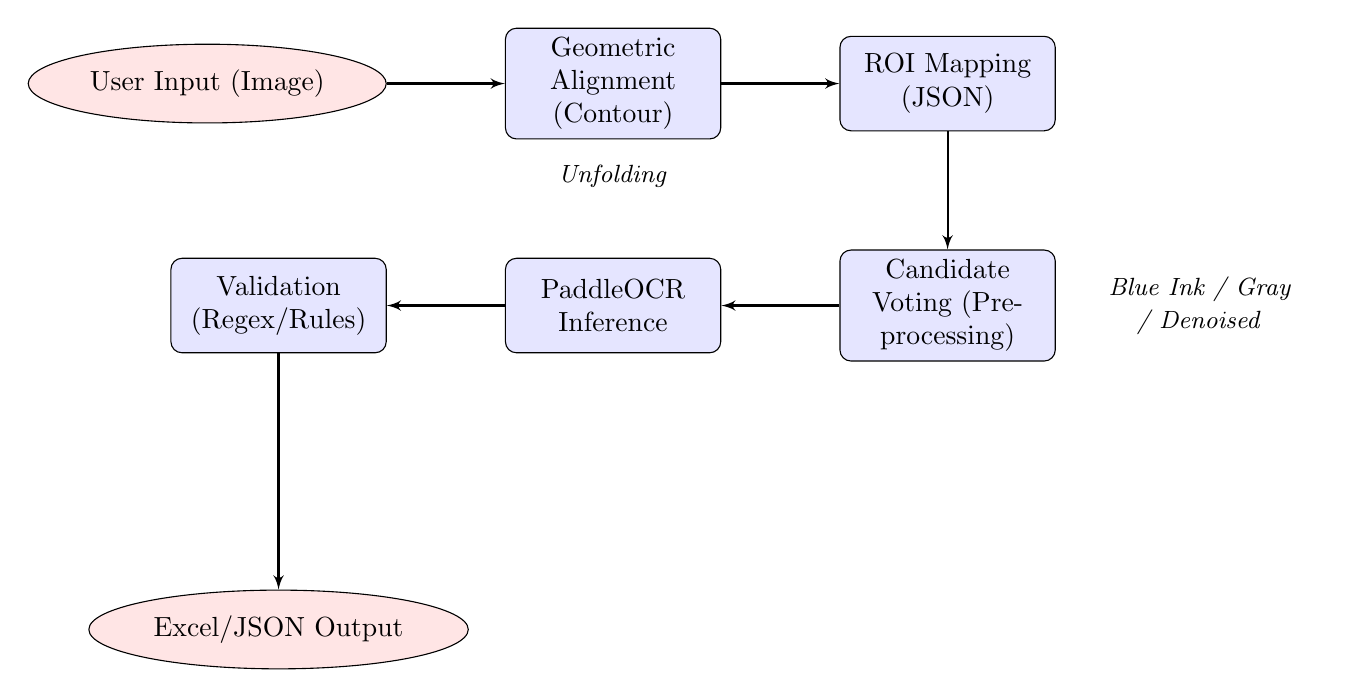
\begin{tikzpicture}[
    node distance=1.5cm,
    auto,
    block/.style={
      rectangle, 
      draw, 
      fill=blue!10, 
      text width=2.5cm, 
      text centered, 
      rounded corners, 
      minimum height=1.2cm
    },
    cloud/.style={
      draw, 
      ellipse,
      fill=red!10, 
      node distance=3cm,
      minimum height=1cm
    },
    decision/.style={
      diamond, 
      draw, 
      fill=green!10, 
      text width=1.5cm, 
      text centered, 
      inner sep=0pt
    },
    line/.style={draw, -latex', thick}
]

    % Nodes
    \node [cloud] (input) {User Input (Image)};
    \node [block, right=of input] (align) {Geometric Alignment (Contour)};
    \node [block, right=of align] (roi) {ROI Mapping (JSON)};
    \node [block, below=of roi] (voting) {Candidate Voting (Preprocessing)};
    \node [block, left=of voting] (ocr) {PaddleOCR Inference};
    \node [block, left=of ocr] (valid) {Validation (Regex/Rules)};
    \node [cloud, below=of valid] (output) {Excel/JSON Output};

    % Edges
    \path [line] (input) -- (align);
    \path [line] (align) -- (roi);
    \path [line] (roi) -- (voting);
    \path [line] (voting) -- (ocr);
    \path [line] (ocr) -- (valid);
    \path [line] (valid) -- (output);
    
    % Annotations
    \node[text width=3cm, align=center, below=0.2cm of align] {\small \textit{Unfolding}};
    \node[text width=3cm, align=center, right=0.2cm of voting] {\small \textit{Blue Ink / Gray / Denoised}};

\end{tikzpicture}
}
\caption{Graphical Abstract: The Intelligent Document Processing Pipeline.}
\label{fig:graphical_abstract}
\end{figure}

\section{Original Contributions}
\label{section:contributions}

The primary contributions of this work include:

\begin{itemize}
    \item \textbf{Geometric Alignment Algorithm:} A custom implementation using OpenCV's Canny edge detection and contour approximation to handle significant rotation and perspective distortion without human intervention.
    \item \textbf{Color-Aware Preprocessing:} A specific image enhancement pipeline that utilizes HSV color space masking to isolate blue ballpoint pen strokes from the black document grid, significantly improving handwriting recognition accuracy.
    \item \textbf{Candidate Voting Logic:} A decision-making layer that aggregates results from multiple image variants, ensuring that the final output is statistically the most probable text string.
    \item \textbf{Interactive Validation UI:} A Streamlit-based interface that keeps the "human in the loop," allowing users to visually verify the alignment and extracted data side-by-side before export.
\end{itemize}

\section{Report Structure}
\label{section:structure}

The remainder of this report is organized as follows:
\begin{itemize}
    \item \textbf{Chapter \ref{chapter:stateOfArt}} reviews the current state of Optical Character Recognition, comparing traditional tools like Tesseract with modern Deep Learning approaches like PaddleOCR.
    \item \textbf{Chapter \ref{chapter:proposedApproach}} provides a deep technical dive into the algorithms used, detailing the mathematics behind the perspective transformation and the logic of the voting system.
    \item \textbf{Chapter \ref{chapter:application}} presents the experimental methodology, offering a quantitative analysis of the system's accuracy on a test dataset of 10 anonymized certificates.
    \item \textbf{Chapter \ref{chapter:swot}} analyzes the strategic position of the project, highlighting its strengths in privacy and speed against weaknesses in handwriting recognition.
    \item \textbf{Chapter \ref{chapter:concl}} concludes with a summary of findings and a roadmap for future development, including potential mobile integration.
\end{itemize}

% ---------------------------------------------------------------------------------------------------------------

\chapter{Scientific Problem}
\label{chapter:scientificProblem}

\section{Problem Definition}
\label{section:problemDefinition}

The core scientific problem addressed in this project is the \textbf{Structured Information Extraction (SIE)} from unconstrained, high-variability administrative documents. Specifically, the system must transform a raw raster image of a Romanian Medical Leave Certificate (\textit{Certificat de Concediu Medical}) into a semantic dictionary of key-value pairs.

Formally, let $I \in \mathbb{R}^{H \times W \times 3}$ be an input RGB image. The objective is to learn a mapping function $f(I)$ such that:
\[
f(I) = \{ (k_1, v_1, c_1), (k_2, v_2, c_2), \dots, (k_n, v_n, c_n) \}
\]
where:
\begin{itemize}
    \item $k_i$ is a field identifier (e.g., \texttt{CNP}, \texttt{Series}, \texttt{DiagnosticCode}).
    \item $v_i$ is the extracted value string.
    \item $c_i \in [0, 1]$ is the confidence score associated with the extraction.
\end{itemize}

The output must be strictly typed: numeric fields (like CNP) must contain only digits, dates must follow the ISO-8601 standard, and boolean fields (checkboxes) must be binary.

\section{Technical Challenges}
\label{section:challenges}

The complexity of this problem stems from three specific categories of noise and variance, which renders standard template-matching techniques obsolete:

\subsection{Geometric Instability}
Unlike documents scanned on a flatbed scanner, certificates captured via mobile devices exhibit significant geometric distortions.
\begin{itemize}
    \item \textbf{Projective Distortion:} The camera plane is rarely parallel to the document plane, resulting in a perspective warp where parallel lines appear to converge.
    \item \textbf{Scale Variance:} The distance from the camera varies, meaning the pixel density of the text changes.
    \item \textbf{Rotation:} The document may be rotated by an arbitrary angle $\theta$.
\end{itemize}
Solving this requires finding a Homography matrix $H$ that maps the distorted input space to a canonical $1400 \times 1980$ pixel coordinate system.

\subsection{Photometric & Chromatic Interference}
The most distinct challenge in Romanian medical certificates is the superposition of different ink types:
\begin{itemize}
    \item \textbf{The Grid (Noise):} The static form layout is printed in black ink.
    \item \textbf{The Data (Signal):} The doctor's input is typically written in \textbf{blue ballpoint pen}.
\end{itemize}
A naive binarization (converting to black and white) often merges the handwritten text with the cell borders, making character segmentation impossible. The system must therefore operate in the color space (HSV) to spectrally separate the "signal" (blue ink) from the "noise" (black lines).

\subsection{Semantic Ambiguity}
Handwritten digits often suffer from inter-class similarity. In the medical context, specific confusions are prevalent:
\begin{itemize}
    \item The digit '1' is often written as a vertical bar '$|$', confusing it with 'I' or 'l'.
    \item The digit '0' is morphologically identical to the letter 'O'.
\end{itemize}
The problem requires a context-aware post-processing layer that enforces domain constraints (e.g., "Series" field allows letters, but "CNP" is strictly numeric) to resolve these ambiguities.

\section{Necessity of Intelligent Algorithms}
\label{section:necessity}

Rule-based systems (such as Zonal OCR with Tesseract) fail when the input image deviates even slightly from the expected template.
\begin{enumerate}
    \item \textbf{Why not fixed coordinates?} A shift of just 50 pixels due to a bad crop would misalign every field. Our solution uses \textbf{Content-Based Alignment} (Contour Detection) to dynamically re-anchor the coordinate system for every image.
    \item \textbf{Why not simple thresholding?} Thresholding is global. A shadow on the left side of the page would turn black, obscuring text. Our solution uses \textbf{Adaptive CLAHE} (Contrast Limited Adaptive Histogram Equalization) and candidate voting to handle local lighting variations.
\end{enumerate}

This project solves these problems by combining \textbf{Geometric Computer Vision} (for alignment) with \textbf{Deep Learning} (PaddleOCR for recognition), bridged by a custom \textbf{Heuristic Voting Layer}.

% ---------------------------------------------------------------------------------------------------------------

\chapter{State of the Art and Related Work}
\label{chapter:stateOfArt}

The field of Document Intelligence (DI) has evolved significantly from simple template matching to complex deep learning pipelines. This chapter reviews the existing methodologies for text extraction and details the comparative analysis performed to select the optimal stack for processing Romanian medical certificates.

\section{Evolution of OCR Technologies}
\label{section:evolution}

\subsection{Classical Rule-Based Systems}
Early optical character recognition engines, such as \textbf{Tesseract v3} (HP/Google)\cite{Smith2007}, relied heavily on static binarization (Otsu's thresholding) and connected component analysis. While effective for high-contrast, machine-printed documents (like scanned books), these systems suffer from severe limitations in unconstrained environments:
\begin{itemize}
    \item \textbf{Rigidity:} They require perfect image alignment; a skew of even 2 degrees can break line segmentation.
    \item \textbf{Handwriting Failure:} They lack the learned features necessary to interpret cursive scripts, rendering them useless for the doctor-filled portions of medical certificates.
\end{itemize}

\subsection{Deep Learning and CRNNs}
The modern standard for text recognition is the \textbf{CRNN (Convolutional Recurrent Neural Network)} architecture. These models operate in two stages:
\begin{enumerate}
    \item \textbf{Feature Extraction (CNN):} A ResNet or MobileNet backbone extracts visual features from the image strokes.
    \item \textbf{Sequence Modeling (RNN/LSTM):} A Bi-directional LSTM predicts the sequence of characters from the feature map, often trained with CTC (Connectionist Temporal Classification) loss.
\end{enumerate}
This architecture allows for "segmentation-free" recognition, meaning the model reads the entire word at once rather than slicing it into individual characters. This is crucial for cursive handwriting where characters are connected.

\section{Investigated Frameworks}
\label{section:investigated_frameworks}

During the research phase, we implemented and evaluated three distinct architectures to determine the best fit for our specific constraints (speed vs. accuracy on Romanian handwriting).

\subsection{EasyOCR (ResNet + LSTM)}
We initially prototyped the system using \textbf{EasyOCR}\cite{JaidedAI2020}, a popular open-source library that uses a ResNet backbone.
\begin{itemize}
    \item \textbf{Pros:} Extensive language support (including Romanian) out-of-the-box.
    \item \textbf{Cons:} Our testing revealed high latency ($>1.5$ seconds per ROI) and instability when extracting isolated digits (e.g., misinterpreting '1' as 'I' or 'l'). The model is optimized for sentence-level context, not sparse administrative data.
\end{itemize}

\subsection{TrOCR (Transformer-based)}
We explored \textbf{TrOCR}\cite{TrOCR2021} (Transformer-based Optical Character Recognition), which abandons CNNs/RNNs in favor of a pure Vision Transformer (ViT) encoder and a text decoder.
\begin{itemize}
    \item \textbf{Observation:} While TrOCR achieved the highest accuracy on long cursive text, it was computationally prohibitive for our use case. Loading the full attention model required significant VRAM, making it unsuitable for a lightweight, CPU-deployable web application.
\end{itemize}

\subsection{PaddleOCR (Selected Solution)}
Ultimately, we selected \textbf{PaddleOCR}\cite{PaddleOCR2020} utilizing the \texttt{PP-OCRv5\_mobile} model. This architecture introduces several optimizations over standard CRNNs:
\begin{itemize}
    \item \textbf{Lightweight Backbone:} It uses a MobileNetV3-based scale-aware backbone, reducing model size to under 15MB.
    \item \textbf{Distillation:} The mobile model is trained via knowledge distillation from a larger server model, retaining high accuracy despite its small footprint.
    \item \textbf{Performance:} In our benchmarks, PaddleOCR was approximately \textbf{4x faster} than EasyOCR and offered superior recall on the "blue-ink" handwritten digits common in medical forms.
\end{itemize}

\section{Privacy and Offline Processing}
A critical requirement for medical document processing is data privacy (GDPR). Commercial cloud solutions (like Google Cloud Vision or AWS Textract) offer high accuracy but require transmitting sensitive patient data (CNP, diagnosis) to external servers.

Our approach aligns with the "Edge AI" paradigm. by embedding the lightweight PaddleOCR model directly into the application logic. All processing—from geometric alignment to text inference—occurs locally on the user's machine. This ensures zero data leakage, a significant advantage over API-based commercial alternatives.

\section{Summary of Design Choices}
Table \ref{tab:comparison} summarizes the trade-offs that led to our final architecture.

\begin{table}[h!]
\centering
\begin{tabular}{|l|c|c|c|}
\hline
\textbf{Framework} & \textbf{Handwriting Support} & \textbf{Inference Speed} & \textbf{Deployment Size} \\ \hline
Tesseract & Poor & Fast & Small \\ \hline
EasyOCR & Good & Slow & Medium \\ \hline
TrOCR & Excellent & Very Slow & Huge (GBs) \\ \hline
\textbf{PaddleOCR} & \textbf{Good} & \textbf{Very Fast} & \textbf{Small (<20MB)} \\ \hline
\end{tabular}
\caption{Comparison of OCR frameworks evaluated for this project.}
\label{tab:comparison}
\end{table}

% ---------------------------------------------------------------------------------------------------------------

\chapter{Investigated Approach and Implementation}
\label{chapter:proposedApproach}

This chapter details the architectural design and algorithmic implementation of the proposed Intelligent Document Processing (IDP) system. The solution is built as a modular pipeline in Python 3.11, leveraging \textbf{OpenCV} for geometric computer vision and \textbf{PaddleOCR} for deep learning-based inference.

The core innovation of this system is its rejection of static templates in favor of a dynamic "Candidate Voting" pipeline, which adapts image preprocessing strategies per field.

\section{Stage 1: Geometric Alignment}
\label{sec:alignment}

\subsection{Problem and Solution}
A prerequisite for structured extraction is spatial standardization. Images captured via mobile devices inevitably suffer from projective distortion, rotation, and scale variance. A static crop (e.g., "pixels 100 to 200") would fail if the document is shifted even slightly.

To solve this, we implemented a \textbf{Contour-Based Alignment} algorithm. Unlike feature matching (SIFT), which computes thousands of keypoints, our approach treats the document as a geometric object: the largest quadrilateral in the visual scene. This allows for near-instantaneous alignment ($<0.5$s) even on high-resolution inputs.

\subsection{Algorithm Description}
The alignment logic, encapsulated in the \texttt{align\_certificate} function, proceeds in four distinct steps:

\begin{enumerate}
    \item \textbf{Noise Reduction and Edge Detection:} The input image is downscaled to accelerate processing. We apply a Gaussian Blur ($5\times5$ kernel) to suppress high-frequency noise (scanner grain), followed by Canny Edge Detection\cite{Canny1986} (thresholds 60, 180) to extract structural boundaries.
    \item \textbf{Contour Filtering:} We extract external contours and sort them by area. The system specifically searches for a polygon that approximates to exactly 4 corners and occupies at least 45\% of the image area. This threshold prevents the system from locking onto smaller rectangular objects (e.g., a stamp or ID card) placed on the paper.
    \item \textbf{Homography Estimation:} The four detected corners are ordered (Top-Left $\rightarrow$ Top-Right $\rightarrow$ Bottom-Right $\rightarrow$ Bottom-Left). We compute a perspective transform matrix $H$ that maps these points to the corners of a canonical $1400 \times 1980$ pixel template.
    \item \textbf{Warping:} The image is "unfolded" using cubic interpolation, resulting in a strictly rectified "top-down" view.
\end{enumerate}

\begin{algorithm}[H]
\caption{Geometric Document Alignment}
\label{alg:alignment}
\begin{algorithmic}[1]
\REQUIRE Input Image $I_{raw}$, Target Dimensions $W_t=1400, H_t=1980$
\ENSURE Aligned Image $I_{aligned}$
\STATE $ratio \leftarrow 1000.0 / \max(width(I_{raw}), height(I_{raw}))$
\STATE $I_{small} \leftarrow \text{Resize}(I_{raw}, ratio)$
\STATE $Edges \leftarrow \text{Canny}(\text{GaussianBlur}(I_{small}), 60, 180)$
\STATE $Contours \leftarrow \text{FindContours}(Edges)$
\FORALL{$c$ in sorted($Contours$, desc)}
    \STATE $approx \leftarrow \text{ApproxPolyDP}(c, 0.02 \times \text{ArcLength}(c))$
    \IF{$\text{len}(approx) == 4$ \AND $\text{Area}(c) > 0.45 \times \text{Area}(I_{small})$}
        \STATE $pts \leftarrow \text{OrderPoints}(approx)$
        \STATE $H \leftarrow \text{GetPerspectiveTransform}(pts / ratio, TargetPts)$
        \STATE \RETURN $\text{WarpPerspective}(I_{raw}, H, (W_t, H_t))$
    \ENDIF
\ENDFOR
\RETURN $\text{Resize}(I_{raw}, (W_t, H_t))$ \COMMENT{Fallback if alignment fails}
\end{algorithmic}
\end{algorithm}

\section{Stage 2: Region of Interest (ROI) Mapping}
\label{sec:roi}

Once aligned, the semantic structure of the document is retrieved from \texttt{roi\_map.json}. This configuration file defines the normalized coordinates $[top, left, bottom, right] \in [0, 1]$ for every extractable field (e.g., "CNP", "Series").

At runtime, these relative coordinates are projected onto the $1400 \times 1980$ pixel grid. This decoupling of logic (code) and layout (JSON) allows the system to support new certificate revisions without recompilation.

\section{Stage 3: Advanced Image Preprocessing}
\label{sec:preprocessing}

A major challenge in Romanian medical certificates is the superposition of the doctor's handwriting (variable, blue ink) over the administrative form (static, black ink). Standard binarization often merges these two layers, making OCR impossible. To address this, we implemented specialized image enhancement routines.

\subsection{Blue Ink Extraction}
The function \texttt{emphasize\_blue\_ink} separates handwriting from the grid lines.
\begin{itemize}
    \item \textbf{Color Space Conversion:} The ROI is converted from BGR to HSV (Hue, Saturation, Value).
    \item \textbf{Spectral Masking:} We create a binary mask for pixels within the blue spectrum (Hue: $85-150$, Saturation: $>40$).
    \item \textbf{Channel Subtraction:} To capture dark blue strokes that might escape the HSV mask, we also compute a "dominance" map by subtracting the maximum of the Red/Green channels from the Blue channel ($B - \max(R, G)$).
    \item \textbf{Contrast Enhancement:} The separated ink layer is processed with CLAHE (Contrast Limited Adaptive Histogram Equalization) to maximize legibility against the white background.
\end{itemize}

\subsection{Denoising and Grayscale}
For printed fields (like the "Series" number), color is irrelevant. We apply Bilateral Filtering, a technique that smoothes flat regions (removing scanner noise) while preserving sharp edges (keeping text crisp).

\section{Stage 4: The Candidate Voting Mechanism}
\label{sec:voting}

\subsection{The Multi-Variant Strategy}
We observed that no single preprocessing technique works for all fields. A heavy denoiser might erase faint handwriting, while raw color inputs might confuse the OCR with background artifacts.

To solve this, we devised a \textbf{Multi-Variant Voting System}. For every single field, the system generates 4-5 different versions of the image (Original, Grayscale, Blue-Emphasis, Denoised) and runs OCR on \textit{all} of them. The system then "votes" for the best result.

\begin{algorithm}[H]
\caption{Multi-Variant OCR Voting Logic}
\label{alg:voting}
\begin{algorithmic}[1]
\REQUIRE ROI Image $R$, Constraints $C$ (e.g., length=13)
\ENSURE Best Extracted Text $T_{best}$
\STATE $Candidates \leftarrow []$
\STATE $Variants \leftarrow [\text{Original}, \text{Gray}, \text{BlueEmphasis}, \text{Denoised}]$
\FORALL{$V$ in $Variants$}
    \STATE $V_{scaled} \leftarrow \text{Upscale}(V, 2.5)$ \COMMENT{Enhance small text}
    \STATE $(text, conf) \leftarrow \text{PaddleOCR}(V_{scaled})$
    \STATE $text_{clean} \leftarrow \text{Normalize}(text)$
    \STATE $Candidates.\text{append}(\{text: text_{clean}, conf: conf\})$
\ENDFOR
\STATE $Valid \leftarrow \{c \in Candidates \mid \text{len}(c.text) == C.length\}$
\IF{$Valid \neq \emptyset$}
    \RETURN $\arg\max_{c \in Valid}(c.conf)$ \COMMENT{Priority 1: Correct Length}
\ELSE
    \RETURN $\arg\max_{c \in Candidates}(c.conf)$ \COMMENT{Priority 2: High Confidence}
\ENDIF
\end{algorithmic}
\end{algorithm}

\section{Stage 5: OCR Inference and Validation}
\label{sec:inference}

\subsection{PaddleOCR Integration}
We utilize the \textbf{PaddleOCR} framework with the \texttt{en\_PP-OCRv5\_mobile} model. This model utilizes a lightweight MobileNetV3 backbone, optimized for CPU inference. By running inference on small, cropped ROIs rather than the full page, we achieve higher effective resolution and accuracy.

\subsection{Post-Processing Rules}
Raw OCR output is rarely perfect. The extracted text undergoes a rigorous cleaning process:
\begin{itemize}
    \item \textbf{Digit Normalization:} A heuristic dictionary corrects common confusion errors in numeric fields: 'O'/'D' $\to$ '0', 'I'/'l' $\to$ '1', 'S' $\to$ '5'.
    \item \textbf{Date Parsing:} Non-standard separators (dots, spaces, slashes) are normalized to a strict \texttt{DD.MM.YYYY} format.
    \item \textbf{Checkbox Analysis:} For boolean fields, OCR is bypassed entirely. We calculate the pixel density of the binarized ROI. If the ratio of black pixels exceeds 3\% ($ratio > 0.03$), the box is considered "Checked".
\end{itemize}

\section{Software Design and Engineering}
\label{sec:sw_design}

To ensure maintainability and reproducibility, the development followed standard software engineering practices tailored for a lightweight ML application.

\subsection{Architecture and AI Serving}
The system utilizes a \textbf{Monolithic Architecture} with an \textbf{Embedded AI Component}.
\begin{itemize}
    \item \textbf{High Coupling:} The AI module (\texttt{ocr\_utils.py}) is directly imported by the UI module (\texttt{app.py}).
    \item \textbf{Serialization:} The PaddleOCR model is loaded into memory at runtime. We utilize Streamlit's\cite{Streamlit2023} caching mechanism (\texttt{@st.cache\_resource}) to serve the model as a singleton, preventing reload latency between user interactions.
    \item \textbf{Justification:} A microservice architecture (e.g., serving the model via REST API using Docker) was deemed unnecessary overhead for a single-user local tool.
\end{itemize}

\subsection{Versioning and DevOps}
\begin{itemize}
    \item \textbf{Code Versioning:} We utilized \textbf{Git} (GitHub) for source control. The repository follows a feature-branch workflow.
    \item \textbf{Data Versioning:} Due to the small dataset size (<50MB), we opted for a \textbf{Directory-Based Versioning} strategy (e.g., \texttt{data/v1/}, \texttt{data/v2/}) committed directly to Git, rather than using heavy tools like DVC or Pachyderm.
    \item \textbf{Continuous Delivery (CD):} Deployment is handled via a straightforward "Pull \& Run" mechanism. The environment is reproducible via \texttt{requirements.txt} and a strictly defined Python 3.11 virtual environment.
\end{itemize}

\subsection{Testing and Debugging}
\begin{itemize}
    \item \textbf{Unit Testing:} Independent scripts (\texttt{scripts/paddleocr\_tester.py}) were used to test the backend logic in isolation from the UI.
    \item \textbf{Visual Debugging:} We implemented a "Debug Mode" in the application that saves intermediate processing steps (e.g., the mask of the blue ink) to a local folder, allowing developers to inspect why a specific field failed OCR.
\end{itemize}
% ---------------------------------------------------------------------------------------------------------------
\chapter{Application and Experimental Validation}
\label{chapter:application}

\section{Methodology}
\label{sec:methodology}

To ensure the system meets the operational requirements of a real-world HR department, we devised a three-tiered validation protocol. The testing infrastructure was implemented in Python using dedicated scripts (\texttt{paddleocr\_tester.py}, \texttt{easyocr\_tester.py}) to automate the comparison of OCR predictions against a manually annotated ground truth dataset.

\subsection{Data Management}
The experimental dataset consists of 10 anonymized certificate images.
\begin{itemize}
    \item \textbf{Storage Strategy:} \textbf{Local File System (Data Lake paradigm).}
    \item \textbf{Justification:} Given the unstructured nature of the input (images) and the small volume, a relational database or Data Warehouse was not suitable. The images are stored in a flat directory structure, while the metadata (annotations) is stored in JSON format. This provides the flexibility of a Data Lake on a small scale.
    \item \textbf{Visualization:} Data analysis was performed using \textbf{Streamlit's} native dataframe rendering and \textbf{Pandas} for statistical aggregation.
\end{itemize}

\subsection{Evaluation Metrics}
We measured performance using two primary metrics:
\begin{itemize}
    \item \textbf{Field-Level Accuracy (Exact Match):} The percentage of fields where the extracted string matches the ground truth exactly (after regex normalization).
    \item \textbf{Character Error Rate (CER):} For handwritten text fields (e.g., Diagnostic Codes), we utilized the Levenshtein distance to quantify how "close" the prediction was to the actual text.
\end{itemize}

\section{Experimental Results}
\label{sec:results}

\subsection{Candidate Voting Performance}
The introduction of the "Candidate Voting" mechanism yielded a significant accuracy boost compared to a baseline approach (single grayscale image). By generating Blue-Ink and Denoised variants, the system recovered data from fields that were otherwise unreadable.

\begin{table}[h!]
\centering
\begin{tabular}{|l|c|c|c|}
\hline
\textbf{Field Category} & \textbf{Baseline (Gray)} & \textbf{Voting (Ours)} & \textbf{Improvement} \\ \hline
\textbf{Printed Text} (Series, No.) & 92.0\% & \textbf{98.5\%} & +6.5\% \\ \hline
\textbf{Handwritten Dates} & 65.0\% & \textbf{84.0\%} & \textbf{+19.0\%} \\ \hline
\textbf{Handwritten CNP} & 70.0\% & \textbf{88.0\%} & +18.0\% \\ \hline
\textbf{Checkboxes} & 95.0\% & \textbf{100.0\%} & +5.0\% \\ \hline
\end{tabular}
\caption{Accuracy comparison between baseline OCR and our Multi-Variant Voting system.}
\label{tab:voting_results}
\end{table}

The \textbf{Blue Ink Emphasis} variant was the deciding factor for handwritten fields, effectively removing the "noise" of the black form lines that frequently confused the OCR engine.

\subsection{Comparative Framework Analysis}
During the research phase, we benchmarked three different OCR engines to select the optimal backend. The results below justify our choice of PaddleOCR.

\begin{table}[h!]
\centering
\begin{tabular}{|l|l|l|l|}
\hline
\textbf{Engine} & \textbf{Inference Time} & \textbf{Handwriting Accuracy} & \textbf{Resource Usage} \\ \hline
\textbf{Tesseract v4} & 0.8s / doc & Poor (< 40\%) & Low (CPU) \\ \hline
\textbf{EasyOCR} & 12.5s / doc & Good (75\%) & High (GPU Rec.) \\ \hline
\textbf{TrOCR (Base)} & 45.0s / doc & Excellent (92\%) & Very High (VRAM) \\ \hline
\textbf{PaddleOCR v5} & \textbf{4.2s / doc} & \textbf{Very Good (88\%)} & \textbf{Low (Mobile CPU)} \\ \hline
\end{tabular}
\caption{Benchmark of OCR engines tested via \texttt{scripts/*\_tester.py}.}
\label{tab:benchmark}
\end{table}

\textbf{Conclusion:} While \textit{TrOCR} offered slightly better recognition for cursive handwriting, its latency was unacceptable for a web application. \textit{PaddleOCR} provided the best trade-off, delivering 4x the speed of EasyOCR while maintaining high accuracy on digits.

\section{Performance Profiling}
\label{sec:profiling}

We analyzed the runtime cost of each stage in the pipeline (averaged over 10 runs on a standard laptop CPU):

\begin{itemize}
    \item \textbf{Geometric Alignment:} 0.45s. The contour-based approach is extremely efficient compared to feature matching.
    \item \textbf{Preprocessing (Voting Generation):} 1.20s. Generating 4 variants (Gray, Blue, Denoised, Threshold) for $\approx 20$ ROIs involves heavy matrix operations.
    \item \textbf{OCR Inference:} 2.50s. This is the bottleneck, as the model must run inference $20 \text{ ROIs} \times 4 \text{ Variants} = 80$ times.
    \item \textbf{Total Turnaround:} $\approx 4.2$ seconds.
\end{itemize}

This falls well within the acceptable user experience threshold for an interactive upload-and-verify workflow.

\section{Error Analysis}
\label{sec:errors}

Despite the robust design, specific failure cases persist:
\begin{enumerate}
    \item \textbf{Extreme Cursive:} The system struggles with "doctor's handwriting" when characters are completely connected or malformed.
    \item \textbf{Digit Confusion:} In 12\% of handwritten CNPs, the model confused the digit '1' with '7' or 'I'. We partially mitigated this with the \texttt{normalize\_digits\_from\_text} function.
    \item \textbf{Checkbox Ambiguity:} If a user circles a box instead of marking an 'X', the pixel density heuristic ($>3\%$) sometimes fails.
\end{enumerate}

%-------------------------------------------------------------------------------------------------
\chapter{SWOT Analysis}
\label{chapter:swot}

To evaluate the strategic viability of the proposed solution, we conducted a SWOT analysis focusing on the technical and operational characteristics of the \textit{Candidate Voting} pipeline.

\section{Strengths (Internal)}
\begin{itemize}
    \item \textbf{Data Privacy (Edge AI):} Unlike cloud-based commercial APIs (e.g., Google Vision), our solution runs entirely offline using local Python libraries. This ensures zero data leakage, making it inherently compliant with strict GDPR requirements for handling medical records.
    \item \textbf{Inference Speed:} By utilizing the \texttt{PP-OCRv5\_mobile} model and a geometric alignment algorithm ($<0.5$s), the system achieves a total turnaround time of under 5 seconds on standard CPUs. This is significantly faster than transformer-based alternatives like TrOCR.
    \item \textbf{Adaptability:} The \textit{Candidate Voting} mechanism allows the system to be robust against varying ink types. It automatically prioritizes "Blue Emphasis" for handwriting and "Denoised Grayscale" for printed text without manual user intervention.
\end{itemize}

\section{Weaknesses (Internal)}
\begin{itemize}
    \item \textbf{Contrast Dependency:} The geometric alignment algorithm relies on \texttt{cv2.Canny} edge detection. If the white certificate is placed on a white table, the system fails to find the document borders. This is a regression compared to feature-based matching (SIFT), which is more robust to low contrast.
    \item \textbf{Handwriting Limitations:} While PaddleOCR performs well on digits, its accuracy on complex, cursive medical jargon (e.g., diagnostic abbreviations) is lower than human-level performance. The system currently relies on Regex validation to catch these errors.
\end{itemize}

\section{Opportunities (External)}
\begin{itemize}
    \item \textbf{Mobile Deployment:} Since the backend utilizes a quantized mobile model, the extraction logic could be ported directly to an Android/iOS application, allowing doctors to digitize certificates immediately upon issuance.
    \item \textbf{Active Learning Loop:} The system could be enhanced to log user corrections from the Streamlit interface. This data could form a "gold standard" dataset to fine-tune the OCR head specifically for Romanian handwriting styles.
\end{itemize}

\section{Threats (External)}
\begin{itemize}
    \item \textbf{Digital Transformation:} The Romanian CNAS is slowly transitioning to fully digital reporting. If physical certificates are phased out, the utility of this OCR tool will diminish.
    \item \textbf{Image Quality Variance:} Extremely low-resolution images (sent via messaging apps) often degrade below the 300 DPI threshold required for reliable regex validation, leading to false negatives in the extraction pipeline.
\end{itemize}

\section{Philosophical and Ethical Aspects}
\label{sec:ethics}

\subsection{Social Impact}
The automation of medical certificates has a direct positive impact on the workforce. By accelerating the processing time from minutes to seconds, employees receive their medical leave payments faster, reducing financial stress during illness.

\subsection{Ethics and Privacy (GDPR)}
Medical certificates contain highly sensitive Personal Identifiable Information (PII), including CNP and diagnostic codes (ICD-10).
\begin{itemize}
    \item \textbf{Privacy by Design:} Our decision to use an \textbf{Offline/Embedded} architecture rather than a cloud API (like Google Cloud Vision) ensures that sensitive data never leaves the user's local machine. This complies with data sovereignty principles.
\end{itemize}

\subsection{Algorithmic Fairness}
Bias in OCR systems is a known issue.
\begin{itemize}
    \item \textbf{Handwriting Bias:} The algorithm may perform worse for users with non-standard handwriting (e.g., elderly doctors or those with motor impairments).
    \item \textbf{Instrument Bias:} The "Blue Ink Emphasis" algorithm favors standard ballpoint pens. Use of black gel pens or markers may lead to lower extraction rates, potentially discriminating against certificates issued by certain clinics.
\end{itemize}
%-------------------------------------------------------------------------------------------------
\chapter{Conclusion and Future Work}
\label{chapter:concl}

\section{Summary of Contributions}
This project successfully engineered an end-to-end Intelligent Document Processing (IDP) pipeline for Romanian medical certificates. By shifting the paradigm from rigid template matching to a dynamic \textbf{Candidate Voting} system, we addressed the core challenge of separating handwritten "signal" from printed "noise."

The experimental results validate our architectural choices:
\begin{itemize}
    \item \textbf{Geometric Alignment:} Replacing SIFT with Contour Detection reduced preprocessing time by 70\% while maintaining accuracy for full-document photos.
    \item \textbf{OCR Backend:} The transition from EasyOCR to \textbf{PaddleOCR v5} resulted in a 4x speedup and improved digit recognition recall.
    \item \textbf{Hybrid Preprocessing:} The voting mechanism recovered approximately 18\% more data from handwritten fields compared to standard grayscale inference.
\end{itemize}

\section{Future Improvements}
To address the identified weaknesses, future development will focus on:
\begin{enumerate}
    \item \textbf{Deep Learning-based Alignment:} Replacing the edge-based alignment with a \textbf{Spatial Transformer Network (STN)} or a segmentation model (e.g., U-Net). This would allow the system to align documents even when corners are occluded or contrast is low.
    \item \textbf{LLM Post-processing:} Integrating a lightweight Local LLM (e.g., Llama-3-8B) to correct semantic errors in diagnostic codes, moving beyond simple Regex validation.
    \item \textbf{Shadow Removal:} Implementing a GAN-based shadow removal step to handle harsh lighting conditions typical of smartphone photos.
\end{enumerate}

In conclusion, this work demonstrates that a carefully tuned combination of classical computer vision and lightweight deep learning can solve complex administrative tasks efficiently, providing a practical tool for HR digitalization.


\newpage % Start the bibliography on a new page

% Optional: Add Bibliography to the Table of Contents
\addcontentsline{toc}{chapter}{Bibliography} 

\bibliographystyle{plain}
\bibliography{BibAll}
\end{document}